\section{Prac 4 - I2C and PWM}
\label{sec:Prac4}
You have been put in charge of implementing ES Games's latest proof of concept for a new gambling machine where users will try and guess a number. Of course, being a sensible individual, you do not condone reckless gambling and know when to draw the line. To this end, you tender your two-week resignation and start looking for a job at a gaming company that better aligns with your values, perhaps \textit{Even Mo' Jang}, \textit{Nin-eleven-do} or  \textit{Beth-Is-Ma}. However as you still have two weeks, your bosses assign your last task to be implementing the logic and user feedback systems.

\subsection{Overview}
You're going to design a simple guessing game with feedback to the user.


A circuit diagram is shown in Figure \ref{fig:P4Circuit} below.

\begin{figure}[H]
\centering
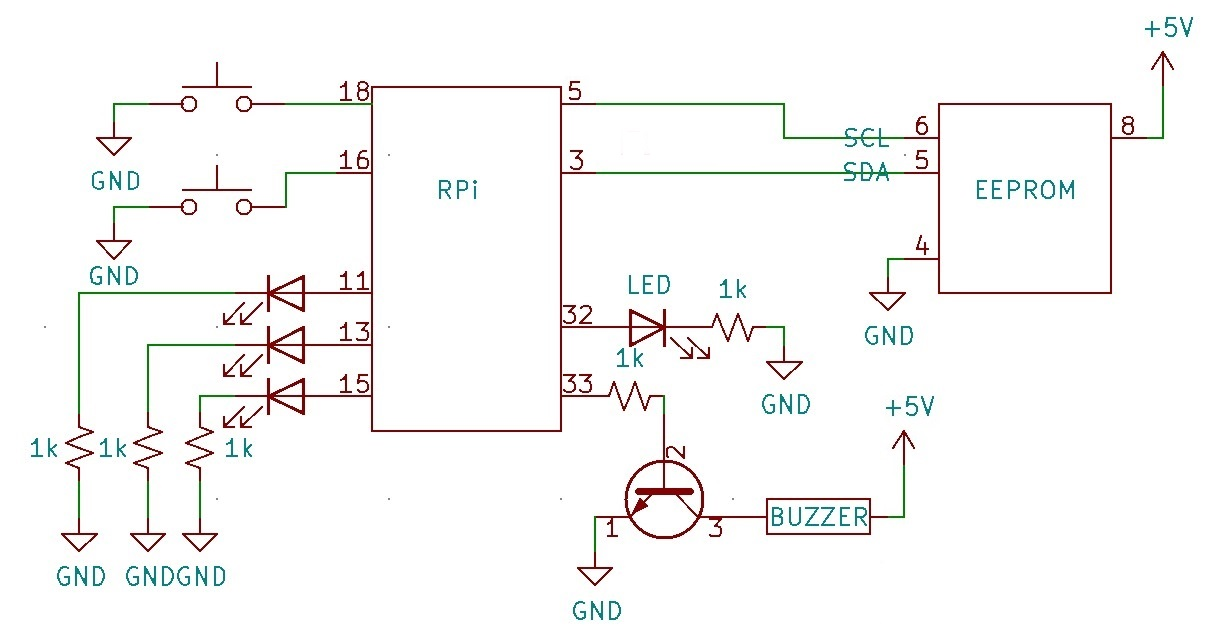
\includegraphics[width=0.8\columnwidth]{Figures/P4Circuit.jpg}
\caption{The circuit diagram for the system}
\label{fig:P4Circuit}
\end{figure}


\subsection{Requirements}
You must do the following:
\begin{itemize}
    \item Use Python 3!
    \item Install libraries as required
    \begin{itemize}
        \item You will need to use pip3, as we're using Python 3\\
        \verb|sudo apt install python3-pip|
        \item You'll need RPi.GPIO for Python 3\\
        \verb|sudo apt-get install python3-rpi.gpio|
        \item You'll need SMBus 2 for Python 3\\
        \verb|sudo pip3 install smbus2|
    \end{itemize}
    \item Read up on the data sheet for the \href{https://datasheet.lcsc.com/szlcsc/Fremont-Micro-Devices-FT24C32A-ETR-T_C232881.pdf}{EEPROM}.
    \item Fetch the prac code off the GitHub repository
\end{itemize}


\subsection{EEPROM}
Read through the data sheet. In order to simplify things for you, an EEPROMUtils library has been provided. The library instantiates an EEPROM class on a specified bus with a defined address. 

Some things you should know about the EEPROM from the datasheet and how the library has been written:
\begin{itemize}
    \item The EEPROM is organised into 128 pages consisting of 32 bytes each.
    \item There are 32768 bits at a word size of 8 bits each, meaning there are 4096 addressable words.
\end{itemize}

The library provided creates a new abstraction called ``blocks":
\begin{itemize}
    \item Each block can be addressed from 0...n, where n is the maximum amount of blocks
    \item Each block consists of 4 words (32 bits)
    \item The write block method will write to as many registers as required by the data passed to it. I.e you can write more than just 4 words using the \verb|write_block| method
\end{itemize}


The following methods are provided:
\begin{itemize}
    \item write block\\
    Writes an array of data starting at the beginning of a particular block
    \item write byte\\
    Writes a singular byte to a given address.
    \item read block\\
    Reads a given amount of registers from the start of a specified block
    \item read byte\\
    Reads a single byte from a specified address.
    \item clear\\
    Writes \verb|0x00| to all memory.
    \item Populate mock scores\\
    Adds 4 mock scores to the EEPROM.
\end{itemize}


\subsection{ASCII}
We can't store text in EEPROM, only 1s and 0s. Thankfully Python will convert numbers between any base, but characters are still unknown. To convert between the two, we can use \verb|ord()| and \verb|chr()| in Python.
\begin{verbatim}
orc(`c') = 99 = 0x63 = 0b01100011
chr(99) = chr(0x63) = chr(0b01100011) = `c'    
\end{verbatim}


\subsection{Design overview}
The requirements of each component and how they respond and are required to act are detailed by comments in the code source.
\begin{enumerate}
    \item Two buttons should be connected, using interrupts and  \href{https://raspberrypi.stackexchange.com/questions/8544/gpio-interrupt-debounce}{debouncing}, which do the following:
        \begin{enumerate}
            \item Button 1 - Increases the user's guess value and update the value shown on the LEDs
            \item Button 2 - Submit the user's guess
        \end{enumerate}
    \item 4 LEDs
    \begin{itemize}
        \item 3 to show the user's current guess value
        \item 1 should show the accuracy of the guess
    \end{itemize}
    \item One Buzzer

\end{enumerate}

\subsection{Playing the game}
When launched, the user is presented with this screen:
\begin{figure}[H]
\centering
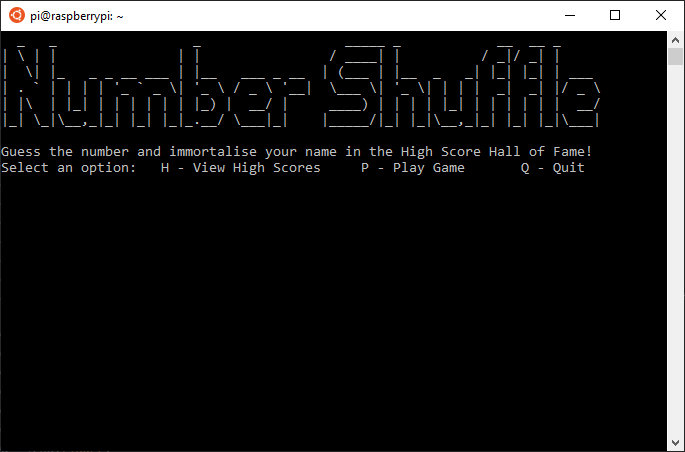
\includegraphics[width=0.7\columnwidth]{Figures/NS_main}
\end{figure}


When the player selects high scores, they should see a screen like this, updated for the latest high scores. Notice how the system knows how many scores are stored but only presents the top three scores.

\begin{figure}[H]
\centering
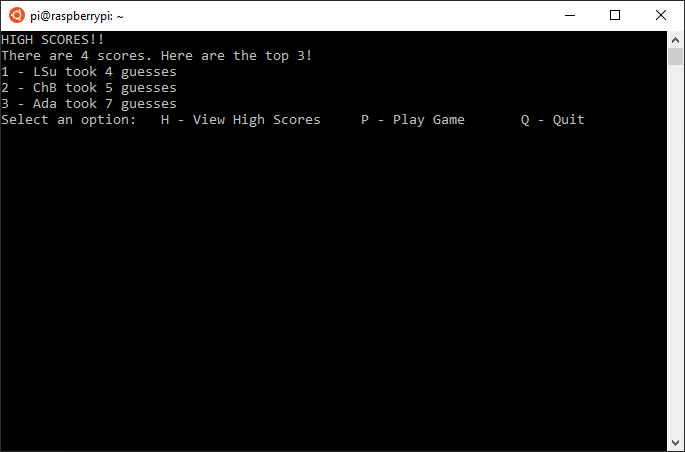
\includegraphics[width=0.7\columnwidth]{Figures/NS_highscores.PNG}
\end{figure}

When a new game is played, this screen is displayed:
\begin{figure}[H]
\centering
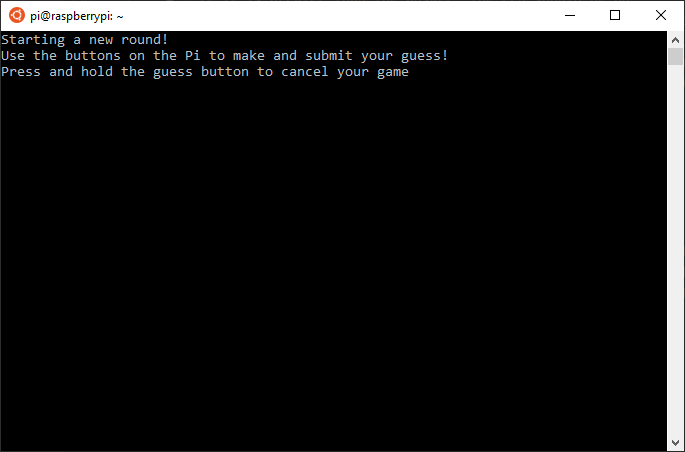
\includegraphics[width=0.7\columnwidth]{Figures/NS_gameplay.PNG}
\end{figure}

Notes on gameplay mechanics are as follows:
\begin{itemize}
    \item At the start of each game, a new random number between 0 and $2^3$ is generated. This is kept secret from the player.
    \item The user presses an ``increase guess" button, and each press updates the value shown on the LEDs.
    \item When the user submits their guess, the PWM LED and the buzzer update appropriately, as described in the P4.py source file.
    \item If the user presses and holds the submit guess button, the buzzer and LEDs are turned off and they are taken back to the main menu
    \item If the user wins by guessing the number correctly, they must be prompted to enter in their name. Your code should handle the scenario that they enter in more than three letters for a name. The system should then store their score to EEPROM and take them back to the main menu.
\end{itemize}

\subsection{Storing Scores}
High scores will be stored on EEPROM with the first byte of the first block storing the amount of scores, and from the first block onwards. An example of this is shown in the figure below.

\begin{figure}[H]
\centering
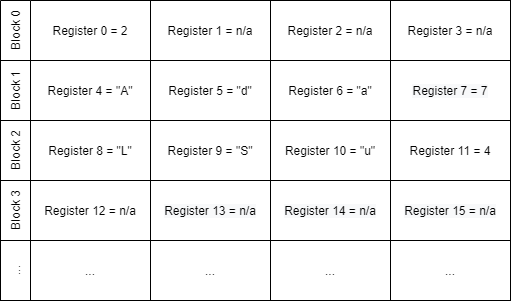
\includegraphics[width=0.7\columnwidth]{Figures/EEPROMBlocks.png}
\end{figure}
It can be seen that the first word in the first block stores the number of scores.
From the first block onwards, we store the scores, with the first three words of a block storing the player's name, and the final word storing how many guesses they took.


\subsection{Walkthrough}
\begin{enumerate}
    \item Start by enabling I2C in raspi-config, under ``Interfacing Options"
    \item Do a git pull in the prac source folder to fetch the Prac 4 content
    \item Build the circuit given to you, taking care not to create any short circuits and configuring things with the correct polarity.
    \item Run \verb|$ sudo i2cdetect -y 1| to see if you can see the EEPROM  on 0x50
    \item Open \verb|p4.py| and write the code required. Some function templates are made available to give you a guide.
    \begin{itemize}
        \item Be sure to take care with regards to which pin numbering is used! The circuit diagram details board mode, not BCM mode! If you chose to make any adjustments, be sure to cater for the new pin numbering.
    \end{itemize}
\end{enumerate}

\subsection{Some Hints}
\begin{enumerate}
    \item You will need to debounce your button presses. The Rpi.GPIO library provides appropriate methods.
    \item The source code provided to you has a lot of implementation in it already. Ensure you read and understand it before embarking out on the practical.
    \item It's important to cleanup the GPIO pins on exit. This has been done for you.
    \item You can use visual studio code or Pycharm Professional (which you can get with a GitHub Education account) to use Python over SSH. This is different from cross-compilation. Guides exist online on how to set this up.
    \item You don't need to edit any code in the EEPROM Utils library, but it does provide some insight into how you might apply some logic! 
\end{enumerate}


\subsection{Deliverables}
At the end of this practical, you must submit a singular PDF, correctly named, with the following each having it's own heading. You do not need to write the report in \LaTeX, but hopefully after Prac 3 you're encouraged by how nice it is to focus on content rather than formatting using a decent text editor! To switch to a single page in \LaTeX from the example source given to you in Prac 3, change the documentclass to ``onecolumn" instead of ``twocolumn". Monospaced text boxes can be created using the \verb|lstlisting| environment.
\begin{enumerate}
    \item A UML use-case diagram of the system. You should know these details from EEE3097S or any design course. If you need a refresher, \href{https://www.youtube.com/watch?v=zid-MVo7M-E}{watch this YouTube Video}.
    \item The Prac4.py code contents
    \begin{itemize}
        \item Each method needs to be in it's own separate text box. 
        \item All the code needs to be included, even if it was a part of the provided code. Do not include the EEPROM library.
        \item Use a monospaced font such as Consolas. Using the correct environment in \LaTeX will do this for you. You can also look into syntax highlighting
    \end{itemize}
\end{enumerate}

Marks will be deducted for not following instructions.